\documentclass[pdf]{beamer}
\usepackage{minted}
\setminted{encoding=utf-8}
\usemintedstyle{colorful}
\usepackage{fontspec}
\usepackage{etoolbox}
\AtBeginEnvironment{minted}{\fontsize{8}{8}\selectfont}
\usepackage{amsmath}
\usepackage{amsfonts}
\usepackage{amssymb}
\usepackage{bm}
\usepackage{graphicx}
\usepackage{subfigure}
\usepackage{outlines}
\usepackage{hyperref}
\usepackage{listings}
\mode<presentation>{\usetheme{}}
\title{Zero to Zipper}
%% \subtitle{}
\author{Slavomir Kaslev \\
  \href{mailto:kaslevs@vmware.com}{kaslevs@vmware.com}}

\begin{document}

\begin{frame}
  \titlepage
\end{frame}

\begin{frame}{QOTD}
  \begin{outline}
    \1 ``The shortest path between two truths in the real domain passes through the complex domain.'' \mbox{Jacques Hadamard}
    \vspace{1cm}
    \1 ``Computer science is no more about computers than astronomy is about telescopes, biology is about microscopes or chemistry is about beakers and test tubes. Science is not about tools, it is about how we use them and what we find out when we do.'' \mbox{Michael R. Fellows} and \mbox{Ian Parberry}
  \end{outline}
\end{frame}

%% \begin{frame}{Why Care about Math?}
%%   \begin{align*}
%%     L(p, \omega_o) = L_e(p, \omega_o) + \int_{S^2} f(p, \omega_o, \omega_i) L(t(p, \omega_i), -\omega_i) \left| \cos \theta_i \right| d \omega_i
%%   \end{align*}
%% \end{frame}

\begin{frame}{The Ocean of Programming Languages}
  \begin{center}
    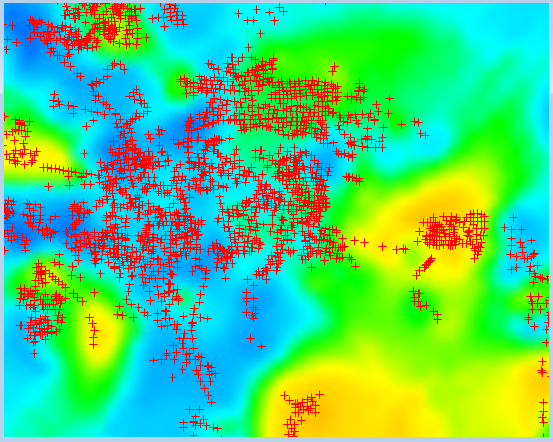
\includegraphics[scale=0.7]{images/points}
  \end{center}
\end{frame}

\begin{frame}{Comparing Core Languages}
  \begin{table}[]
    \noindent
    \begin{tabular}{|l|l|l|}
      \hline
      \textbf{C}  & \textbf{Haskell}  & \textbf{Lean} \\
      \hline
      data Expr   & data Expr         & data Expr     \\
      data Type   & data Type         &               \\
      data Stmt   &                   &               \\
      \hline
    \end{tabular}
  \end{table}
\end{frame}

\begin{frame}[fragile]{C Core Language 1/3}
  \begin{minted}[escapeinside=~~,mathescape=true]{Haskell}
data Expr
  = Comma       [Expr]
  | Assign      AssignOp Expr Expr
  | Cond        Expr (Maybe Expr) Expr
  | Binary      BinaryOp Expr Expr
  | Cast        Type Expr
  | Unary       UnaryOp Expr
  | SizeofExpr  Expr
  | SizeofType  Type
  | Index       Expr Expr
  | Call        Expr [Expr]
  | Member      Expr Ident Bool
  | Var         Ident
  | Const       Constant
  | CompoundLit Type InitializerList
  \end{minted}
\end{frame}

\begin{frame}[fragile]{C Core Language 2/3}
  \begin{minted}[escapeinside=~~,mathescape=true]{Haskell}
data Type
  = VoidType
  | BoolType
  | CharType
  | IntType
  | FloatType
  | DoubleType
  | ShortType   Type
  | LongType    Type
  | SignedType  Type
  | UnsigType   Type
  | SUType      StructureUnion
  | EnumType    Enumeration
  | FunPtr      Type [Type]
  | Ptr         Type
  | Arr         Type ArraySize
  | TypeDef     Ident
  \end{minted}
\end{frame}

\begin{frame}[fragile]{C Core Language 3/3}
  \begin{minted}[escapeinside=~~,mathescape=true]{Haskell}
data Stmt
  = Label Ident Stmt [Attribute]
  | Case Expr Stmt
  | Default Stmt
  | Expr (Maybe Expr)
  | Compound [Ident] [CompoundBlockItem]
  | If Expr Stmt (Maybe Stmt)
  | Switch Expr Stmt
  | While Expr Stmt Bool
  | For (Either (Maybe Expr) Type)
        (Maybe Expr)
        (Maybe Expr)
        Stmt
  | Goto Ident
  | Cont
  | Break
  | Return (Maybe Expr)
  \end{minted}
\end{frame}

\begin{frame}[fragile]{Haskell Core Language}
  \begin{minted}[escapeinside=~~,mathescape=true]{Haskell}
data Expr b
  = Var   Id
  | Lit   Literal
  | App   (Expr b) (Arg b)
  | Lam   b (Expr b)
  | Let   (Bind b) (Expr b)
  | Case  (Expr b) b Type [Alt b]
  | Tick  (Tickish Id) (Expr b)
  | Type  Type
  | Cast  (Expr b) Coercion
  | Coercion Coercion

data Type
  = TyVarTy   Var
  | LitTy     TyLit
  | AppTy     Type Type
  | ForAllTy  !TyCoVarBinder Type
  | FunTy     Type Type
  | TyConApp  TyCon [KindOrType]
  | CastTy    Type KindCoercion
  | CoercionTy Coercion
  \end{minted}
\end{frame}

\begin{frame}{The Duality of Code and Data}
  \begin{center}
    
\includegraphics[scale=0.35]{images/yin-yang}
  \end{center}
  %% \vspace{1cm}
  %% \tiny{Ostermann, Klaus \& Jabs, Julian. (2018). Dualizing Generalized Algebraic Data Types by Matrix Transposition}
\end{frame}

%% \begin{frame}{The Configuration Complexity Clock\footnotemark[1]\hspace*{1pt}}
%%   \begin{center}
%%     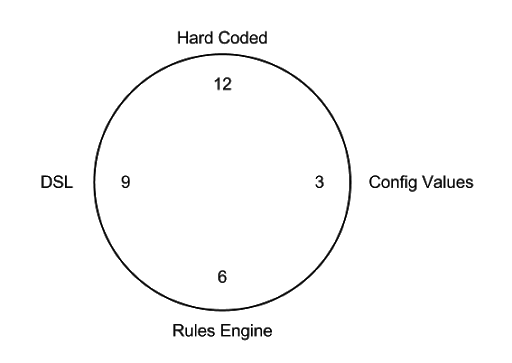
\includegraphics[scale=0.50]{images/ConfigurationComplexityClock}
%%   \end{center}
%%   \footnotetext[1]{\url{http://mikehadlow.blogspot.com/2012/05/configuration-complexity-clock.html}}
%% \end{frame}

%% \begin{frame}{The Duality of Algebra and Geometry}
%%   \begin{table}[]
%%   \noindent
%%     \begin{tabular}{ll}
%%       \hline
%%       Algebra     & Geometry    \\
%%       \pause
%%       Left Brain  & Right Brain \\
%%       \pause
%%       Code        & Data        \\
%%       \hline
%%     \end{tabular}
%%   \end{table}
%%   \begin{outline}
%%     \1``‘Should you just be an algebraist or a geometer?’ is like saying ‘Would you rather be deaf or blind?’'' \mbox{Sir Michael Francis Atiyah}
%%     \1``Bad programmers worry about the code. Good programmers worry about data structures and their relationships.'' \mbox{Linus Torvalds}
%%   \end{outline}
%% \end{frame}

\begin{frame}[fragile]{Lean Core Language}
  \begin{minted}[escapeinside=@@,mathescape=true]{Lean}
inductive expr
| var         : nat → expr
| sort        : level → expr
| const       : name → list level → expr
| mvar        : name → name → expr → expr
| local_const : name → name → binder_info → expr → expr
| app         : expr → expr → expr
| lam         : name → binder_info → expr → expr → expr
| pi          : name → binder_info → expr → expr → expr
| elet        : name → expr → expr → expr → expr
| macro       : macro_def → list expr → expr
  \end{minted}
\end{frame}

\begin{frame}{The Curry-Howard Correspondence Extended\footnotemark[3]}
  \begin{center}
    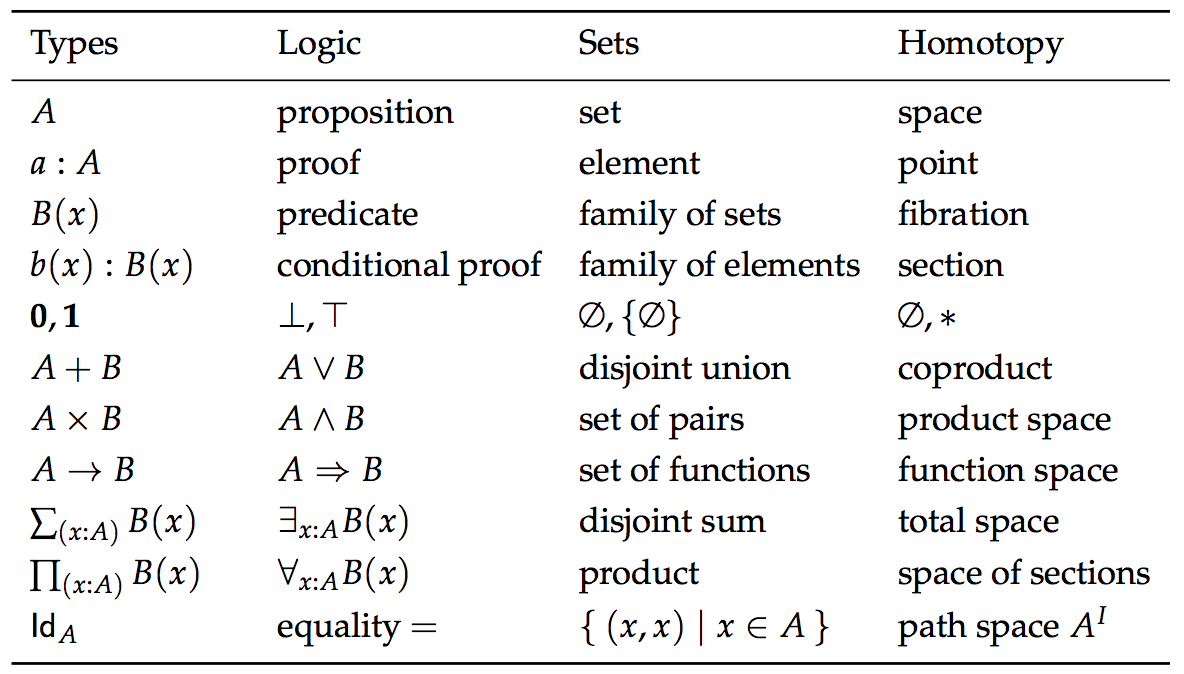
\includegraphics[scale=0.47]{images/hott}
  \end{center}
  \footnotetext[3]{\url{http://saunders.phil.cmu.edu/book/hott-online.pdf\#page=23}}
\end{frame}

\begin{frame}{The Elephant}
  \begin{center}
    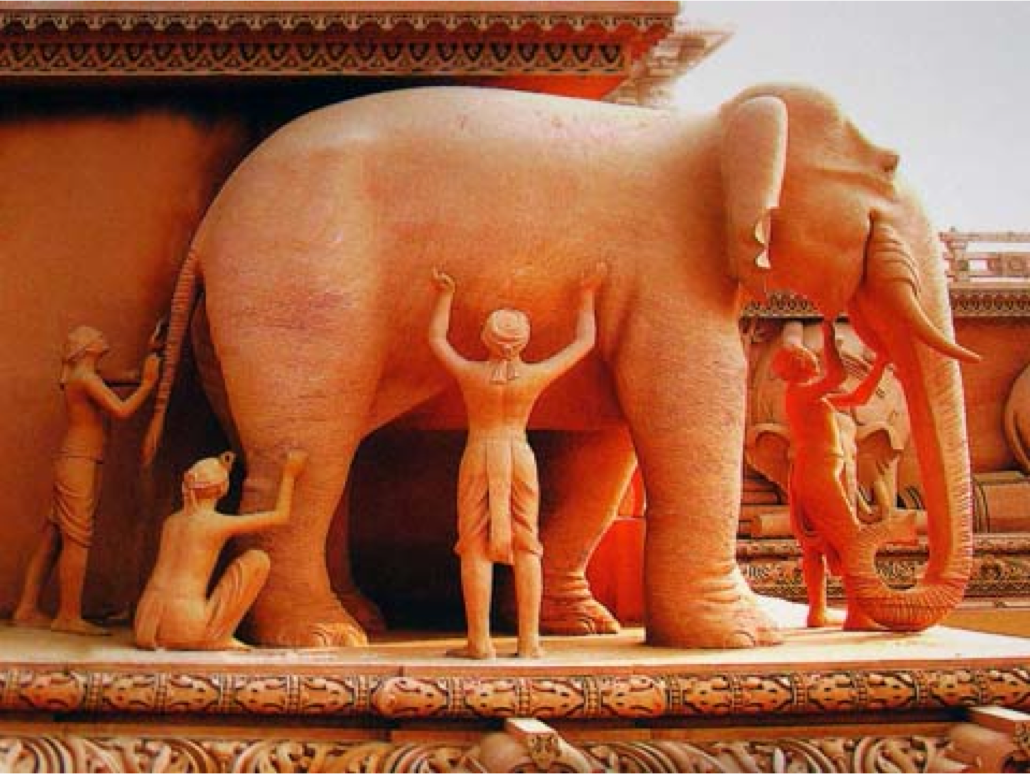
\includegraphics[scale=0.28]{images/elephant}
  \end{center}
\end{frame}

\begin{frame}[fragile]{Isomorphisms in Haskell}
  \begin{minted}[escapeinside=~~,mathescape=true]{Haskell}
data Iso a b = Iso { f :: a -> b, g :: b -> a }
-- Should satisfy the following laws:
--   $\forall$ x : a, g (f x) = x
--   $\forall$ x : b, f (g x) = x

inv :: Iso a b -> Iso b a
inv (Iso f g) = Iso g f

comp :: Iso a b -> Iso b c -> Iso a c
comp (Iso f1 g1) (Iso f2 g2) = Iso (f2 . f1) (g1 . g2)
  \end{minted}
\end{frame}

\begin{frame}[fragile]{Isomorphisms in Lean}
  \begin{minted}[escapeinside=@@,mathescape=true]{Lean}
structure iso (a b : Type) :=
(f : a → b) (g : b → a) (gf : Π x, g (f x) = x) (fg : Π x, f (g x) = x)

def inv {a b} (i : iso a b) : iso b a :=
@$\langle$@i.g, i.f, i.fg, i.gf@$\rangle$@

def comp {a b c} (i : iso a b) (j : iso b c) : iso a c :=
@$\langle$@j.f @$\circ$@ i.f, i.g @$\circ$@ j.g, by simp [j.gf, i.gf], by simp [i.fg, j.fg]@$\rangle$@
  \end{minted}
\end{frame}

\begin{frame}{Type Sizes}
  \begin{outline}
    \1 Suppose there's a size function for \textit{finite} types $|\cdot| : Type \to \mathbb{N}$ and let's look at the sizes of the fundamental types namely
    \begin{align*}
      A \oplus B \hspace{1cm} A \otimes B \hspace{1cm} A \to B
    \end{align*}
    \1 One can prove that
    \begin{align*}
      |A \oplus B| &= |A| + |B| \\
      |A \otimes B| &= |A| \cdot |B| \\
      |A \to B| &= |B|^{|A|}
    \end{align*}
  \end{outline}
\end{frame}

\begin{frame}{From Isomorphisms to Equations and Back}
  \begin{outline}
    \1 Let $|A| = a$, $|B| = b$ and $|C| = c$
    \1 Distributive Law
    \begin{align*}
      A \otimes (B \oplus C) &= (A \otimes B) \oplus (A \otimes C) \\
      a(b+c) &= a b + a c
    \end{align*}
    \1 Pattern matching on disjoint union
    \begin{align*}
      A \oplus B \to C &= (A \to C) \otimes (B \to C) \\
      c^{a+b} &= c^{a} c^{b}
    \end{align*}
    \1 Function currying
    \begin{align*}
      A \to B \to C &= A \otimes B \to C \\
      c^{b^{a}} &= c^{a b}
    \end{align*}
  \end{outline}
\end{frame}

\begin{frame}{Analytic Combinatorics}
  \begin{outline}
    \1 Analytic combinatorics deals with counting combinatorial objects by means of their generating functions
    \1 What is a generating function?
    \1 Given a type $A$ and a size function $|\cdot| : A \to \mathbb{N}$, $A$'s ordinary generating function (OGF) is defined as
    \begin{align*}
      A(x) = \sum_{a : A}{x^{|a|}} = \sum_{n=0}^{\infty}{a_n x^n}
    \end{align*}
    \1 The numbers $a_n$ tell us how many objects in $A$ are of size $n$
  \end{outline}
\end{frame}

\begin{frame}[fragile]{Symbolic Method: Finding generating functions}
  \begin{outline}
    \1 Flajolet and Sedgewick propose a simple method of finding equation for the OGF of a given combinatorial construction expressed in their specification language
    \1 In the special case of algebraic data types, the symbolic method uses the fact that if $A, B, C$ are types and $A(x), B(x), C(x)$ are the corresponding OGFs then
    \begin{align*}
      C = A \oplus B &\implies C(x) = A(x) + B(x) \\
    \text{and} \\
      C = A \otimes B &\implies C(x) = A(x) B(x)
    \end{align*}
  \end{outline}
\end{frame}

\begin{frame}[fragile]{Symbolic Method: Examples 1/2}
  \begin{minted}[escapeinside=~~,mathescape=true]{Haskell}
    data Maybe x = None | Just x
  \end{minted}
  \begin{align*}
    M(x) &= 1 + x
  \end{align*}

  \begin{minted}[escapeinside=~~,mathescape=true]{Haskell}
    data List x = Nil | Cons x (List x)
  \end{minted}
  \begin{align*}
    L(x) &= 1 + x L(x)
  \end{align*}
  \begin{align*}
    L(x) &= \frac{1}{1-x}
  \end{align*}
  \begin{align*}
    L(x) &= 1 + x + x^2 + x^3 + x^4 + x^5 + \ldots
  \end{align*}
\end{frame}

\begin{frame}[fragile]{Symbolic Method: Examples 2/2}
  \begin{minted}[escapeinside=~~,mathescape=true]{Haskell}
    data C x = Single x | Pair x x
    type F x = [C x]
  \end{minted}
  \begin{align*}
    F(x) &= \frac{1}{1 - x - x^2}
  \end{align*}
  \begin{align*}
    F(x) &= 1 + x + 2 x^2 + 3 x^3 + 5 x^4 + 8 x^5 + 13 x^6 + 21 x^7 + \ldots
  \end{align*}
  \begin{minted}[escapeinside=~~,mathescape=true]{Haskell}
    data BinTree x = Leaf | Branch x (BinTree x) (BinTree x)
  \end{minted}
  \begin{align*}
    B(x) &= 1 + x B(x)^2 \\
    B(x) &= \frac{1 - \sqrt{1 - 4x}}{2x}
  \end{align*}
  \begin{align*}
    B(x) &= 1 + x + 2x^2 + 5x^3 + 14x^4 + 42x^5 + 132x^6 + 429x^7 + \ldots
  \end{align*}
\end{frame}

\begin{frame}{Zipper}
  \begin{outline}
    \1 Zipper of a data structure is another data structure that provides iteration and modification in $O(1)$ time complexity
    \1 OGF for the zipper over any data structure with OGF $F(x)$ is defined as
    \begin{align*}
      Z_F(x) &= x \frac{\partial}{\partial{x}}F(x)
    \end{align*}
    \1 The derivative of an OGF $\frac{\partial}{\partial{x}}F(x)$ gives the OGF of the same structure with one hole in it, e.g.
    \begin{align*}
      \frac{\partial}{\partial{x}}x^n &= n x^{n-1}
    \end{align*}
    \1 The $x$ in the right hand side is called focus and holds what was initially in that hole
  \end{outline}
\end{frame}

\begin{frame}[fragile]{List Zipper 1/2}
  \begin{minted}[escapeinside=~~,mathescape=true]{Haskell}
    data List x = Nil | Cons x (List x)
  \end{minted}
  \begin{align*}
    L(x) &= 1 + xL(x)
  \end{align*}
  \begin{align*}
    L(x) &= \frac{1}{1-x}
  \end{align*}
  \begin{align*}
    \frac{\partial}{\partial{x}}L(x) &= \frac{1}{(1-x)^2} = L(x)^2
  \end{align*}
  \begin{align*}
    Z_L(x) &= x L(x)^2
  \end{align*}
  \begin{minted}[escapeinside=~~,mathescape=true]{Haskell}
    data ZList x = Focus x (List x) (List x)
  \end{minted}
\end{frame}

\begin{frame}[fragile]{List Zipper 2/2}
  \begin{minted}[escapeinside=~~,mathescape=true]{Haskell}
data ZList a = Focus a [a] [a]

toZipper :: [a] -> Maybe (ZList a)
toZipper [] = Nothing
toZipper (x:xs) = Just $ Focus x xs []

fromZipper :: ZList a -> [a]
fromZipper   (Focus x r []) = x:r
fromZipper z@(Focus x r (y:p)) = fromZipper $ left z

set :: ZList a -> a -> ZList a
set (Focus x r p) y = Focus y r p

left :: ZList a -> ZList a
left z@(Focus x r []) = z
left   (Focus x r (y:p)) = Focus y (x:r) p

right :: ZList a -> ZList a
right z@(Focus x [] p) = z
right   (Focus x (y:r) p) = Focus y r (x:p)

main = do
  let z  = fromJust $ toZipper [1,2,3,4,5]
      z1 = set (right $ right z) 42
      z2 = set (left z1) 0
  print $ fromZipper z2
-- prints [1,0,42,4,5]
  \end{minted}
\end{frame}

\begin{frame}[fragile]{Binary Tree Zipper 1/3}
  \begin{minted}[escapeinside=~~,mathescape=true]{Haskell}
    data BinTree x = Leaf | Branch x (BinTree x) (BinTree x)
  \end{minted}
  \begin{align*}
    B(x) &= 1 + x B(x)^2
  \end{align*}
  \begin{align*}
    \frac{\partial}{\partial{x}}B(x) &= B(x)^2 + 2 x B(x) \frac{\partial}{\partial{x}}B(x)
  \end{align*}
  \begin{align*}
    \frac{\partial}{\partial{x}}B(x) &= \frac{B(x)^2}{1 - 2 x B(x)}
  \end{align*}
  \begin{align*}
    Z_B(x) &= x B(x)^2 \frac{1}{1 - 2 x B(x)}
  \end{align*}
  \begin{minted}[escapeinside=~~,mathescape=true]{Haskell}
    data Segment x = SLeft x (BinTree x) | SRight x (BinTree x)
    data ZBinTree x = Focus x (BinTree x) (BinTree x) [Segment x]
  \end{minted}
\end{frame}

\begin{frame}[fragile]{Binary Tree Zipper 2/3}
  \begin{minted}[escapeinside=~~,mathescape=true]{Haskell}
data BinTree a = Leaf | Branch a (BinTree a) (BinTree a)

data Segment a = SLeft a (BinTree a) | SRight a (BinTree a)
data ZBinTree a = Focus a (BinTree a) (BinTree a) [Segment a]

toZipper :: BinTree a -> Maybe (ZBinTree a)
toZipper Leaf = Nothing
toZipper (Branch x l r) = Just $ Focus x l r []

fromZipper :: ZBinTree a -> BinTree a
fromZipper   (Focus x l r []) = Branch x l r
fromZipper z@(Focus x l r (s:p)) = fromZipper $ up z

set :: ZBinTree a -> a -> ZBinTree a
set (Focus x l r p) y = Focus y l r p

left :: ZBinTree a -> ZBinTree a
left z@(Focus x Leaf r p) = z
left   (Focus x (Branch y ll lr) r p) = Focus y ll lr (SLeft x r:p)

right :: ZBinTree a -> ZBinTree a
right z@(Focus x l Leaf p) = z
right   (Focus x l (Branch y rl rr) p) = Focus y rl rr (SRight x l:p)

up :: ZBinTree a -> ZBinTree a
up z@(Focus x l r []) = z
up   (Focus x l r (SLeft y ur:p))  = Focus y (Branch x l r) ur p
up   (Focus x l r (SRight y ul:p)) = Focus y ul (Branch x l r) p
  \end{minted}
\end{frame}

\begin{frame}[fragile]{Binary Tree Zipper 3/3}
  \begin{minted}[escapeinside=~~,mathescape=true]{Haskell}
t :: BinTree Int
t = Branch 1 (Branch 2 Leaf (Branch 3 Leaf (Branch 4 Leaf Leaf)))
             (Branch 5 Leaf Leaf)

main = do
  let z  = fromJust $ toZipper t
      z1 = set (right $ left z) 42
      z2 = set (up z1) 0
  print $ fromZipper z2

-- prints
-- Branch 1 (Branch 0 Leaf (Branch 42 Leaf (Branch 4 Leaf Leaf)))
--          (Branch 5 Leaf Leaf)
  \end{minted}
\end{frame}

\begin{frame}[fragile]{Challenge}
  \begin{outline}
    \1 Write a library that automatically derives the zipper and its operations for any given data structure
    \vspace{5mm}
    \begin{minted}[escapeinside=~~,mathescape=true]{Haskell}
      data RoseTree a = Node a [RoseTree a]
      $(mkZipper ''RoseTree)
    \end{minted}
    \vspace{3mm}
    \2 Bonus points if it also derives a \lstinline{Comonad} instance
    \vspace{1cm}
    \1 To handle multiple type variables the zipper can be generalized
    \begin{align*}
      Z_F(\bm{x}) &= \bm{x} \cdot \nabla F(\bm{x})
    \end{align*}
  \end{outline}
\end{frame}

\begin{frame}{Further Reading}
  \small
  \begin{outline}
    \1 ``Functional Pearl: The Zipper'' by \mbox{G\'erard Huet}
    \1 ``The Derivative of a Regular Type is its Type of One-Hole Contexts'' by \mbox{Conor McBride}
    \1 ``Analytic Combinatorics'' course on Coursera \url{https://www.coursera.org/learn/analytic-combinatorics}
    \1 ``An Introduction to the Analysis of Algorithms'' by \mbox{Philippe Flajolet} and \mbox{Robert Sedgewick}
    \1 ``Analytic Combinatorics'' by \mbox{Philippe Flajolet} and \mbox{Robert Sedgewick}
    \1 ``Homotopy Type Theory: Univalent Foundations of Mathematics'' by \mbox{The Univalent Foundations Program}
    \1 ``Constructive Mathematics and Computer Programming'' by \mbox{Per Martin-L\"{o}f}
    \1 Tangent bundle \url{https://en.wikipedia.org/wiki/Tangent_bundle}
    \1 Code and slides from this talk \url{https://github.com/skaslev/zero-to-zipper}
  \end{outline}
\end{frame}

\begin{frame}{Thank you}
\end{frame}

\end{document}
